% 简略版：问题、方法、过程、结论（给自己快速过一遍用）
\documentclass[a4paper,zihao=5,fontset=fandol,UTF8]{ctexart}
\usepackage[a4paper,left=2.5cm,right=2.5cm,top=2.2cm,bottom=2.2cm]{geometry}
\usepackage{fontspec}
\setmainfont{texgyretermes}[Extension=.otf,UprightFont=*-regular,BoldFont=*-bold,ItalicFont=*-italic,BoldItalicFont=*-bolditalic]
\usepackage{graphicx,booktabs,enumitem}
\graphicspath{{figures/}}
\linespread{1.3}
\setlength{\parskip}{3pt}
\setlist{nosep,leftmargin=*,labelindent=2em}
\ctexset{section={format=\large\bfseries\heiti\raggedright, beforeskip=10pt, afterskip=4pt, name={,、}, number=\chinese{section}}}
\pagestyle{plain}

\begin{document}
\begin{center}
{\Large\bfseries\heiti 上大校园猫捉老鼠：躲还是跑？——简略版}\\[4pt]
{\small 刘明洋\quad 24121874\quad 《博弈论与强化学习》算法实战报告}
\end{center}

\section{问题}
上海大学逐浪徒步社团在 A–G 楼一带组织了一次 30 人的猫捉老鼠：10 只猫、20 只老鼠，上下两轮各 30 分钟，碰到就算抓到，被抓的老鼠变成猫，不能进楼，开局在 C、D、CJ、DJ 楼之间集合。实战里活得最久的人都是躲出来的，鼠王躲在空调外机和墙之间的夹缝里，一直到最后都没被抓到；猫有时围捕，有时单追；夜跑的路人常被错当成猫。本文回答五个问题：
\begin{enumerate}[label=（\arabic*）]
  \item 躲为什么比跑好？靠的是“站着不动不显眼”，还是“藏身处不显眼”？
  \item 哪里最好躲？
  \item 第一轮看到结果后，第二轮会不会从跑转向躲？会不会反过来？
  \item 只奖励“活得久”的 AI 老鼠，会不会自己学会躲？藏身处不再隐蔽时，它会不会改成跑？
  \item 不写围捕规则，猫能不能自己学会围捕？个人奖励和团队奖励哪个更好？
\end{enumerate}

\section{方法}
\textbf{场地}：从 OpenStreetMap（二维地图）下载上大宝山校区，截取 A–GJ 楼一带 418 m × 526 m，按 0.5 m 一格分成平地、教学楼、灌木丛、空调外机夹缝四类。OSM 里没有空调外机的数据，所以按固定随机种子沿楼外墙放置，平均每 14 m 一台。

\textbf{博弈}：30 人的部分可观测随机博弈，被抓即转化。每个人只能看到 20 m 内、没被楼挡住的人；猫每秒按一定速率“发现”老鼠，走动比站着显眼 4 倍，灌木丛里再降到 1/5，夹缝里降到 1/20。

\textbf{反事实对照}：现实中藏身处当然更隐蔽。把某个“不显眼”系数改成 1，是为了看“没有这一条，躲还剩多少优势”，从而找出躲为什么有效。

\textbf{三类实验}：脚本策略（五种老鼠同局配对比较）；上下两轮模仿（费米规则，每人看同局一个同伴）；猫鼠用 PPO 共同训练（猫的五种奖励：个人、团队、混合、按参与分配、随机分配；隐蔽无优势；历史对手池与只用最新对手，共八组，各 3 个种子）。

\section{过程}
\begin{enumerate}[label=（\arabic*）]
  \item 先在 50 m 小场地上做机制探针，期间 AI 老鼠找到了两个环境漏洞，修好后结论才稳定。
  \item 真实地图上脚本策略 6 组条件各 256 局；随机藏身点 512 局；两轮模仿 5 种比例各 256 局；共同训练 24 个模型（普通组 300 轮，对手池组 600 轮），每个 64 局交叉评估。脚本实验的置信区间按局自举，强化学习先抽种子再抽局（分层自举）。
  \item 所有图用 Times New Roman + 宋体，按 Nature 规范通过对齐、字号、重叠三项检查。
\end{enumerate}

\section{结论}
\begin{enumerate}[label=（\arabic*）]
  \item \textbf{躲确实更好}：一轮 30 分钟里，躲平均活 11.2 分钟，跑 5.4 分钟；只躲夹缝 11.1 分钟，与躲相当。
  \item \textbf{优势主要来自藏身处本身}：取消地形的隐蔽优势后，躲只比跑多 0.6 分钟；两项都取消只多 0.3 分钟（不显著）；只取消“静止不显眼”仍多 3.7 分钟。
  \item \textbf{好藏身点要“藏得住、走得到”}：随机分配时灌木和夹缝差不多安全（9.3 和 9.6 分钟）；夹缝赢在紧贴每栋楼。
  \item \textbf{两轮之间双向转化}：躲在任何比例下都多活 4.5–5.5 分钟，但只看一个同伴时，四分之一人躲的情况下 15\% 跑者改躲、34\% 躲者改跑；运气掩盖了差距，躲的比例每轮只升 0.01–0.02。
  \item \textbf{AI 老鼠学到的是针对对手的对策}：换成脚本猫后只活 4.3 分钟，不如脚本跑者。历史对手池比只用最新对手好（4.8 对 2.3 分钟），但仍远不如脚本躲者。取消隐蔽优势后几乎不再进夹缝（18\% → 5\%），也没有“都改成跑”。
  \item \textbf{团队平分奖励让猫变弱}：脚本老鼠对上团队奖励的猫活 16.2 分钟，对上个人奖励的猫 8.6 分钟；功劳只分给在场的猫时恢复到 9.3 分钟；同样多的功劳随机分时最弱（20.3 分钟），说明关键是奖励要落到出力的猫身上。这类猫更爱扎堆，抓得却最少。
\end{enumerate}

\textbf{局限}：发现系数按体验设定；空调外机位置是合成的；每组 3 个种子，种子之间差别大，强化学习结论是探索性的；“按参与分配”不是严格的差分奖励。

\vspace{4pt}
\begin{center}
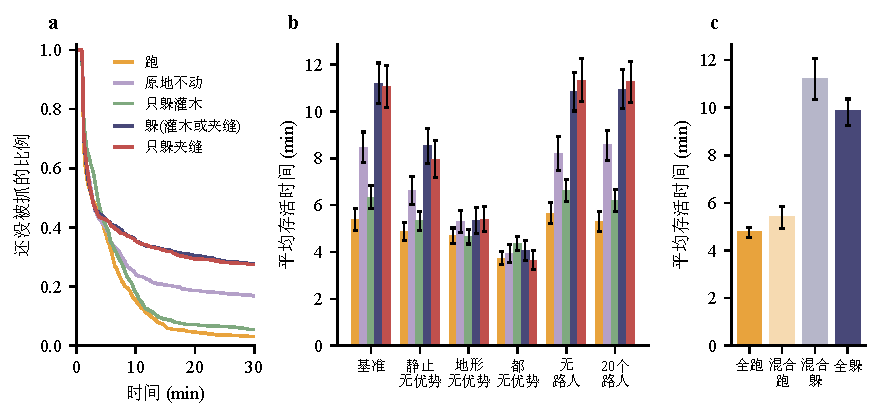
\includegraphics[width=0.95\textwidth]{fig3_campus_hide_vs_run.pdf}\\[-2pt]
{\small 真实地图上各策略的存活：\textbf{a} 存活曲线；\textbf{b} 六种条件下的平均存活（地形无优势时躲的优势大部分消失）；\textbf{c} 同质与混合群体。}
\end{center}
\end{document}
